\subsection{Sincronia}

Os contadores síncronos são aqueles em que todas as mudanças de estado ocorrem simultaneamente, ou seja, todos os flip-flops são acionados pelo mesmo sinal de clock. 

\begin{figure}[htbp]
   	\centering
   	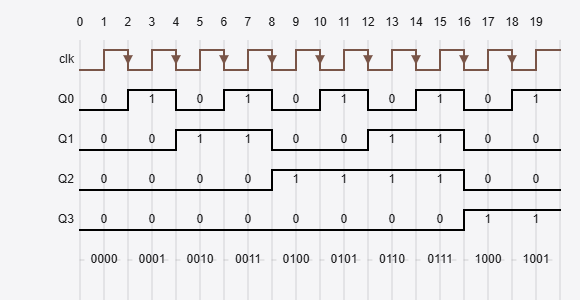
\includegraphics[width=0.7\linewidth]{images/sincrono-time-diagram.png}
  	 \caption{Diagrama de tempo de um contador síncrono}
   	\label{fig:sincrono-time-diagram}
\end{figure}

Já os contadores assíncronos, também conhecidos como contadores ripple, têm seus flip-flops acionados em cascata, o que pode levar a atrasos na propagação do sinal.

\begin{figure}[htbp]
   	\centering
   	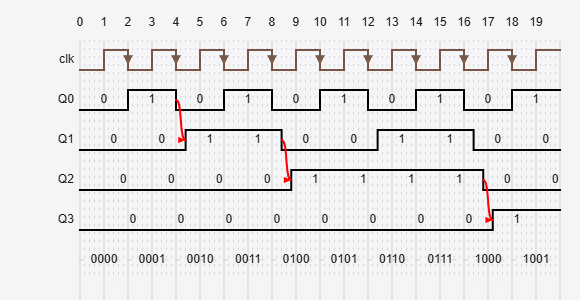
\includegraphics[width=0.7\linewidth]{images/assincrono-time-diagram.png}
  	 \caption{Diagrama de tempo de um contador assíncrono}
   	\label{fig:assincrono-time-diagram}
\end{figure}

Apesar da aparente hierarquia entre estes dois tipos, contadores assíncronos costumam aumentar a complexidade do circuito para cada bit adicional armazenado. 
Mesmo assim, eles são preferidos em aplicações que exigem alta velocidade e precisão, como em sistemas de temporização e contagem de eventos.

Tipicamente, contadores assíncronos são implementados utilizando flip-flops JK ou D em cascata seguindo o seguinte modelo:

\begin{figure}[htbp]
   	\centering
   	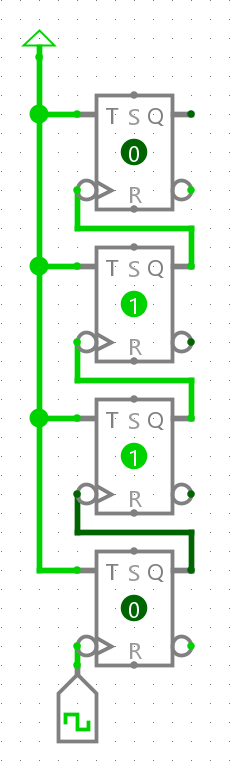
\includegraphics[width=0.2\linewidth]{images/assincrono-circuit.png}
  	 \caption{Circuito de um contador assíncrono}
   	\label{fig:assincrono-circuit}
\end{figure}

Enquanto os contadores síncronos costumam ser modelados como FSMs, com funções de transição $\delta$ de estado bem definidas:

\begin{figure}[htbp]
   	\centering
   	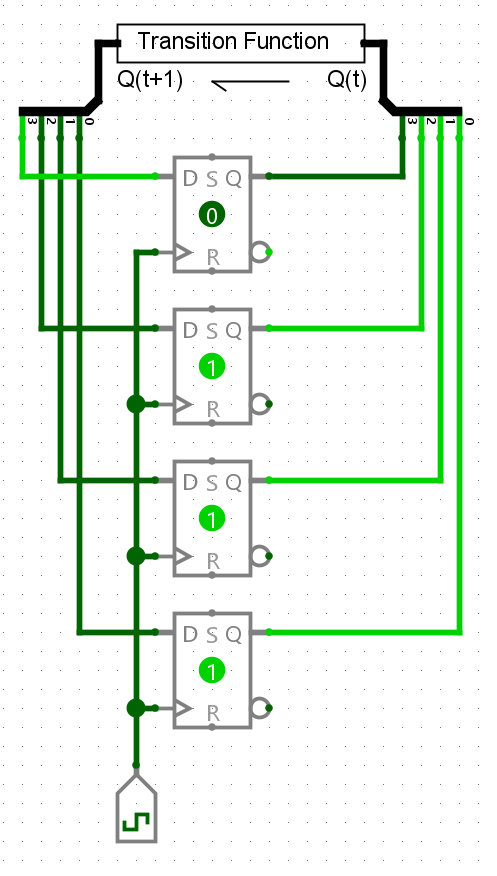
\includegraphics[width=0.4\linewidth]{images/sincrono-circuit.png}
  	 \caption{Circuito de um contador síncrono}
   	\label{fig:sincrono-circuit}
\end{figure}

Esta propriedade de sincronização torna os contadores síncronos mais adequados para aplicações que exigem precisão e confiabilidade. 
Além disso,o fato de $\delta$ ser uma função determinística por natureza de implementação, torna os contadores síncronos adequados para aplicações personalizadas. 
